\section{Results}\label{sec:results}

\subsection{The acceptance task at the default number of frames}

Table~\ref{tab:main} gives the main comparison on the acceptance task with \parFrames{} frames over \nSeedsTwo{} seeds, and Fig.~\ref{fig:curves} shows the intensity of the lowest moving trap along one sequence.

\begin{table}[t]
\centering\small
\caption{Acceptance task, \parFrames{} frames, \nSeedsTwo{} seeds: transient minimum ratio of the moving traps (mean and 95 percent interval of the mean), per-frame minimum ratio (median), largest phase step (maximum over the seeds), largest per-frame spread (median over the seeds), seconds per sequence (median) and the reading of the benchmark rule against the flicker-bounded sequence on the dip.}
\label{tab:main}
\adjustbox{max width=\textwidth}{\begin{tabular}{@{}l r r r r r r@{}}
\toprule
Sequence & Transient minimum ratio, mean (95\% interval) & Per-frame minimum ratio & Largest phase step (rad) & Largest frame $\sigma$ (\%) & Seconds & Reading against the flicker-bounded sequence \\
\midrule
flicker-bounded sequence & 0.923 (0.916 to 0.930) & 0.987 & 0.077 & 0.24 & 1.19 &  \\
linear phase interpolation & 0.644 (0.584 to 0.703) & 0.652 & 0.476 & 23.50 & 1.63 & proposed ($n$ = 6, 6) \\
per-frame GS with phase induction, 5 iterations & 0.948 (0.929 to 0.966) & 0.973 & 0.408 & 2.23 & 0.59 & published ($n$ = 6, 6) \\
per-frame GS with phase induction, 10 iterations & 0.925 (0.890 to 0.961) & 0.981 & 0.619 & 1.29 & 0.94 & tie ($n$ = 6, 6) \\
\bottomrule
\end{tabular}
}
\end{table}

\begin{figure}[t]
\centering
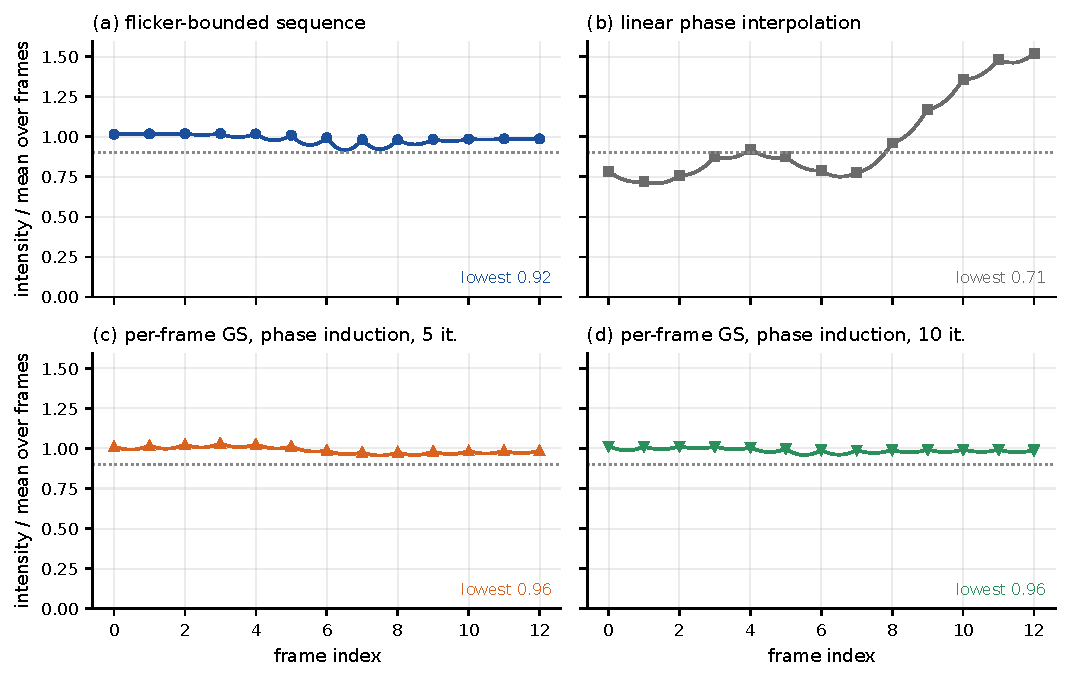
\includegraphics[width=\textwidth]{fig-curves.pdf}
\caption{Intensity of the lowest moving trap of each method, divided by its mean over the frames, along the \parFrames{}-frame acceptance sequence of the first seed: frames are the markers and the lines between them are the blend of two holograms. The dotted line is $0.9$. Linear phase interpolation (b) dips and overshoots; the three optimized sequences (a, c, d) stay close to one, and the per-frame sequences show small steps at the frames.}
\label{fig:curves}
\end{figure}

For the sequence the lowest transient ratio of the moving traps is a mean of \accBTransMean{} (standard deviation \bTwoSd{}, interval \accBTransCiLo{} to \accBTransCiHi{}, median \accBTransMed{}, range \accBTransMin{} to \accBTransMax{}), above $0.9$ on every seed. Linear phase interpolation has a mean of \accLpiTransMean{} (standard deviation \lpiSd{}, interval \accLpiTransCiLo{} to \accLpiTransCiHi{}, range \accLpiTransMin{} to \accLpiTransMax{}), below $0.9$ on every seed. The paired difference of Eq.~\ref{eq:paired} has a mean of \diffTwoMean{} with a 95 percent interval of \diffTwoCiLo{} to \diffTwoCiHi{}, so the interval excludes zero, and the benchmark rule reads the dip as \readThirteenLpiDip{} for the sequence ($n$ = \readThirteenLpiDipN). The per-frame spread differs by a factor of \sigmaFrameFactorLo{} to \sigmaFrameFactorHi{}: the largest per-frame relative standard deviation is at most \bTwoSigmaFrame{} percent for the sequence (median \bTwoSigmaFrameMed{}) and between \lpiSigmaFrameMin{} and \lpiSigmaFrameMax{} percent for linear phase interpolation (median \lpiSigmaFrameMed{}), because its intermediate frames are not optimized.

The per-frame Gerchberg--Saxton sequence with phase induction at \parKimIters{} iterations per frame reaches a higher minimum than the proposed sequence: a mean of \accKimFiveTransMean{} (interval \accKimFiveTransCiLo{} to \accKimFiveTransCiHi{}, range \accKimFiveTransMin{} to \accKimFiveTransMax{}) against \accBTransMean{}, a gap of \dipGap{} in the mean, and the benchmark rule reads the dip as \readThirteenKimFiveDip{} ($n$ = \readThirteenKimFiveDipN). On every seed the published method is above the proposed sequence on this measure. At equal work, \parFrameIters{} iterations per frame, its mean is \accKimTenTransMean{} (interval \accKimTenTransCiLo{} to \accKimTenTransCiHi{}) and the rule reads a \readThirteenKimTenDip{}. So the finding for the dip is: the proposed sequence is well above linear phase interpolation, below the published per-frame method at its own iteration count, and indistinguishable from it at ten iterations per frame. On the per-frame spread the reading is \readThirteenKimFiveSigma{} for the sequence against the per-frame method at \parKimIters{} iterations and \readThirteenKimTenSigma{} at ten: its frames are better equalized, with a median largest spread of \accBSigmaMed{} percent against \accKimFiveSigmaMed{} and \accKimTenSigmaMed{} percent.

\begin{table}[t]
\centering\small
\caption{The time profile of the sequence as a parameter, a comparison added after the results, acceptance task, \parFrames{} frames, \readProfileN{} seeds: transient minimum ratio (mean and 95 percent interval), largest phase step (maximum over seeds), largest per-frame spread (median) and the reading of the benchmark rule against each baseline on the dip, for the default minimal-jerk profile and for the linear profile of the baselines.}
\label{tab:profile}
\adjustbox{max width=\textwidth}{\begin{tabular}{@{}l r r r l l l@{}}
\toprule
Time profile of the sequence & Transient minimum ratio, mean (95\% interval) & Largest phase step (rad) & Largest frame $\sigma$ (\%) & Reading against per-frame GS, 5 iterations & Against 10 iterations & Against linear phase interpolation \\
\midrule
minimal-jerk (the default) & 0.923 (0.916 to 0.930) & 0.077 & 0.24 & published ($n$ = 6, 6) & tie ($n$ = 6, 6) & proposed ($n$ = 6, 6) \\
linear (the baselines' profile) & 0.967 (0.960 to 0.974) & 0.086 & 0.21 & proposed ($n$ = 6, 6) & proposed ($n$ = 6, 6) & proposed ($n$ = 6, 6) \\
\bottomrule
\end{tabular}
}
\end{table}

Table~\ref{tab:profile} reports both time profiles against every baseline. With the default minimal-jerk profile the rule reads the dip as \readProfileDefaultKimFiveDip{} against the per-frame method at \parKimIters{} iterations, as a \readProfileDefaultKimTenDip{} at \parFrameIters{} iterations and as \readProfileDefaultLpiDip{} against linear phase interpolation. With the linear profile it reads \readProfileLinearKimFiveDip{} against the per-frame method at \parKimIters{} iterations, \readProfileLinearKimTenDip{} at \parFrameIters{} and \readProfileLinearLpiDip{} against linear phase interpolation, on the dip and on the per-frame spread alike, with a mean of \ablTLinearMean{} against \accKimFiveTransMean{}. The deficit of the default profile has a cause that the data locate: at \parFrames{} frames its peak shift between frames is \accPeakStep{} Fourier units, outside the method's own step bound of \claimStepFu{} Fourier units, for which the bound asks \accFramesForMove{} frames, while the constant-velocity profile at the same frame count has a smaller peak shift for the same move. The default therefore runs outside the bound that the paper derives, and the comparison at this frame count sets the sequence outside its design condition against baselines inside theirs. At 25 frames, inside the bound, the default ties both per-frame sequences (Table~\ref{tab:frames}).

\subsection{Number of frames}

\begin{table}[t]
\centering\small
\caption{Transient minimum ratio of the moving traps (median and range over \nSeedsTwo{} seeds) and per-frame minimum ratio (median) of the four sequences on the acceptance task at 7, \parFrames{} and 25 frames.}
\label{tab:frames}
\adjustbox{max width=\textwidth}{\begin{tabular}{@{}l l r r r r@{}}
\toprule
Frames & Sequence & Transient minimum ratio, median & Range & Per-frame minimum ratio, median & $n$ \\
\midrule
13 & flicker-bounded sequence & 0.923 & 0.915 to 0.932 & 0.987 & 6 \\
13 & linear phase interpolation & 0.648 & 0.551 to 0.709 & 0.652 & 6 \\
13 & per-frame GS with phase induction, 5 iterations & 0.953 & 0.918 to 0.965 & 0.973 & 6 \\
13 & per-frame GS with phase induction, 10 iterations & 0.926 & 0.880 to 0.966 & 0.981 & 6 \\
7 & flicker-bounded sequence & 0.754 & 0.735 to 0.766 & 0.986 & 6 \\
7 & linear phase interpolation & 0.621 & 0.479 to 0.666 & 0.663 & 6 \\
7 & per-frame GS with phase induction, 5 iterations & 0.896 & 0.877 to 0.903 & 0.976 & 6 \\
7 & per-frame GS with phase induction, 10 iterations & 0.868 & 0.794 to 0.895 & 0.975 & 6 \\
25 & flicker-bounded sequence & 0.973 & 0.963 to 0.977 & 0.988 & 6 \\
25 & linear phase interpolation & 0.648 & 0.576 to 0.722 & 0.651 & 6 \\
25 & per-frame GS with phase induction, 5 iterations & 0.970 & 0.934 to 0.980 & 0.972 & 6 \\
25 & per-frame GS with phase induction, 10 iterations & 0.949 & 0.891 to 0.982 & 0.981 & 6 \\
\bottomrule
\end{tabular}
}
\end{table}

\begin{figure}[t]
\centering
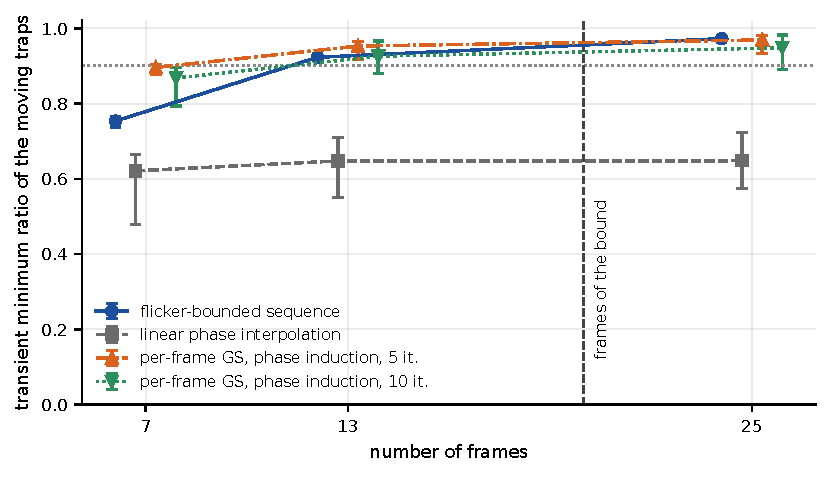
\includegraphics[width=\textwidth]{fig-frames.pdf}
\caption{Transient minimum ratio of the moving traps against the number of frames of the acceptance task for the four sequences; markers are medians over \nSeedsTwo{} seeds and bars are the range. The dotted line is $0.9$ and the dashed vertical line is the number of frames that the bound of Eq.~\ref{eq:frames} requires for this move.}
\label{fig:frames}
\end{figure}

Table~\ref{tab:frames} and Fig.~\ref{fig:frames} vary the number of frames. With 7 frames the sequence reaches a median of \bTwoMedSeven{} (minimum \bTwoMinSeven), below $0.9$ on every seed, linear phase interpolation \lpiMedSeven{}, and the per-frame method at \parKimIters{} iterations \readSevenKimFiveDip{} by the rule and at ten iterations \readSevenKimTenDip{}: with few frames the induced sequence is clearly better than the proposed one, which is consistent with the frame-count equation, because the move of two Fourier units needs \accFramesForMove{} frames for the step bound and 7 frames give a peak step of \fpeval{round(15/8*\accFu/(7-1)/\claimStepFu,1)} times the bound. With 25 frames, above the bound for this move, the sequence reaches a median of \bTwoMedTwentyFive{} (minimum \bTwoMinTwentyFive), linear phase interpolation \lpiMedTwentyFive{}, and the reading against both per-frame sequences is a \readTwentyFiveKimFiveDip{} and a \readTwentyFiveKimTenDip{}. The proposed sequence thus gains more from extra frames than linear phase interpolation, which does not improve, and catches up with the per-frame method; the per-frame method is the better choice when the number of frames is small and the two are equivalent on this measure when it is large. The per-frame minimum ratio, without the blend, is above $0.97$ for the sequence and the per-frame sequences at all three counts, so the dips of the first three are produced by the transition between frames and not by the frames.

\subsection{Phase continuity}

\begin{figure}[t]
\centering
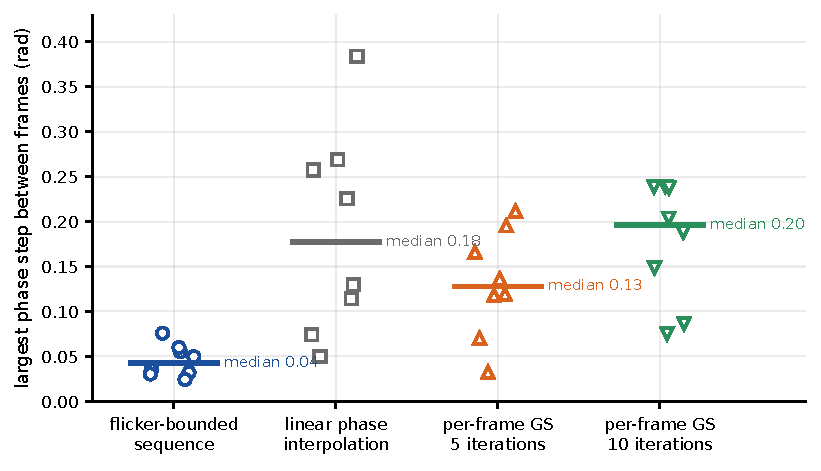
\includegraphics[width=\textwidth]{fig-steps.pdf}
\caption{Largest phase step between consecutive frames of each of the eight moving traps of the acceptance task (first seed), for the four sequences. Each marker is one trap and the horizontal lines are the medians over the traps, lowest for the sequence. The ranges of the traps overlap between methods, so the comparison of the text rests on the largest step of each seed (Table~\ref{tab:main}), which is at the top of each column.}
\label{fig:steps}
\end{figure}

Figure~\ref{fig:steps} shows the quantity that the lock is designed to control, the largest phase step $\Theta$ of Eq.~\ref{eq:phasestep}. Over the \nSeedsTwo{} seeds of the acceptance task the largest phase step of the sequence is \accBStepMax{} rad (mean \accBStepMean{}, interval \accBStepCiLo{} to \accBStepCiHi{}). The per-frame method at \parKimIters{} iterations has \accKimFiveStepMax{} rad (mean \accKimFiveStepMean{}), a factor of \stepRatio{}; at ten iterations it has \accKimTenStepMax{} rad, a factor of \stepRatioTen{}; and linear phase interpolation has \accLpiStepMax{} rad, a factor of \stepRatioLpi{}. The sequence has the smaller step on every one of the \nSeedsTwo{} seeds against the per-frame method at \parKimIters{} iterations, and the same holds at 7 and 25 frames. Two readings of these numbers are limited. The step of linear phase interpolation is not small even though its interpolated phase is linear, because the phase achieved in a frame that is an inverse transform of interpolated spots is not the interpolated one. And the largest step of the induced sequence, \accKimFiveStepMax{} rad, is about \fpeval{round(\accKimFiveStepMax/pi,2)}$\pi$, below the several tenths of $\pi$ at which Knottnerus et al.\ saw no change in atom survival~\cite{lpi}: the measurements do not show that the induced sequence would lose atoms. The advantage of the lock is a margin on a quantity that matters near $\pi$, and the acceptance task does not approach it.

\subsection{Long moves and the sort of a \texorpdfstring{$6\times6$}{6 by 6} array}

\begin{table}[t]
\centering\small
\caption{Transient minimum ratio of the moving traps on the long lattice moves ($\longSeeds$ seeds) and on the sort of the $6\times6$ array ($\cTenSeeds$ seeds), each at the frames of the bound: median and range over seeds, seeds at $0.9$ or above, and the reading of the benchmark rule against the flicker-bounded sequence.}
\label{tab:long}
\adjustbox{max width=\textwidth}{\begin{tabular}{@{}l r l r r r r@{}}
\toprule
Move & Frames & Sequence & Median & Range & Seeds at 0.9 or above & Reading against the flicker-bounded sequence \\
\midrule
lattice, 12 bins & 58 & flicker-bounded sequence & 0.933 & 0.023 to 0.965 & 6 of 8 &  \\
lattice, 12 bins & 58 & linear phase interpolation & 0.675 & 0.568 to 0.756 & 0 of 8 & proposed ($n$ = 8) \\
lattice, 12 bins & 58 & per-frame GS with phase induction, 5 iterations & 0.960 & 0.927 to 0.976 & 8 of 8 & tie ($n$ = 8) \\
lattice, 12 bins & 58 & per-frame GS with phase induction, 10 iterations & 0.948 & 0.912 to 0.978 & 8 of 8 & tie ($n$ = 8) \\
lattice, 20 bins & 95 & flicker-bounded sequence & 0.936 & 0.584 to 0.966 & 6 of 8 &  \\
lattice, 20 bins & 95 & linear phase interpolation & 0.651 & 0.581 to 0.701 & 0 of 8 & proposed ($n$ = 8) \\
lattice, 20 bins & 95 & per-frame GS with phase induction, 5 iterations & 0.960 & 0.928 to 0.976 & 8 of 8 & published ($n$ = 8) \\
lattice, 20 bins & 95 & per-frame GS with phase induction, 10 iterations & 0.949 & 0.908 to 0.979 & 8 of 8 & tie ($n$ = 8) \\
rearrangement C10, 16 moving traps & 137 & flicker-bounded sequence & 0.914 & 0.909 to 0.917 & 6 of 6 &  \\
rearrangement C10, 16 moving traps & 137 & linear phase interpolation & 0.556 & 0.044 to 0.738 & 0 of 6 & proposed ($n$ = 6) \\
rearrangement C10, 16 moving traps & 137 & per-frame GS with phase induction, 5 iterations & 0.938 & 0.922 to 0.956 & 6 of 6 & published ($n$ = 6) \\
rearrangement C10, 16 moving traps & 137 & per-frame GS with phase induction, 10 iterations & 0.920 & 0.846 to 0.936 & 5 of 6 & tie ($n$ = 6) \\
\bottomrule
\end{tabular}
}
\end{table}

\begin{figure}[t]
\centering
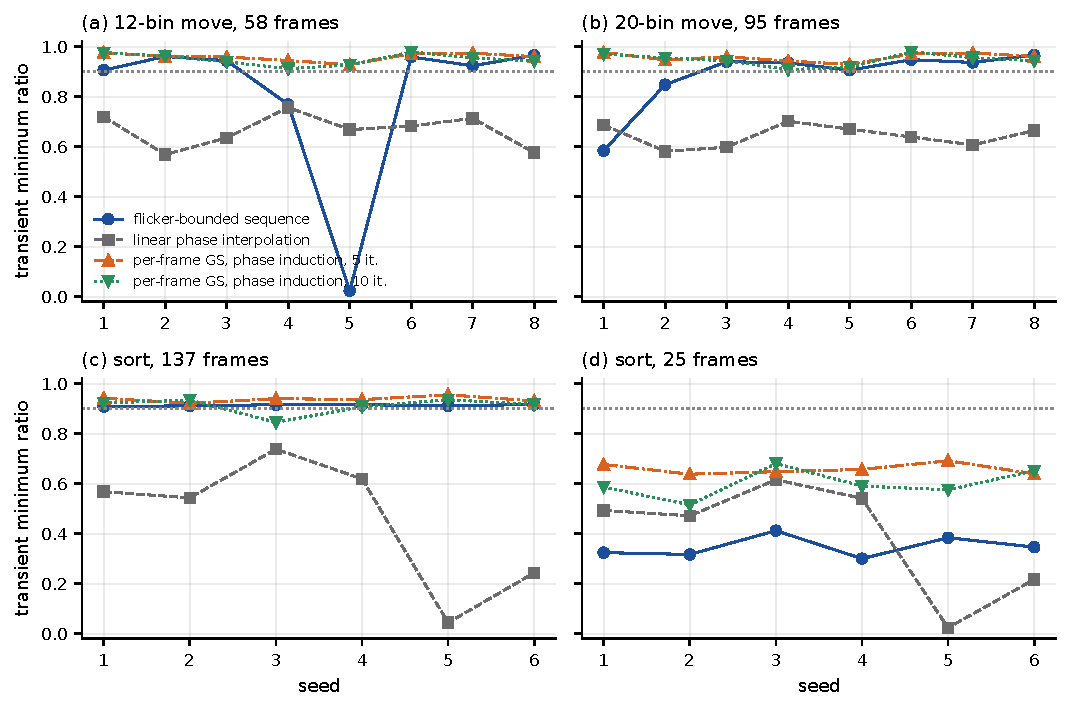
\includegraphics[width=\textwidth]{fig-long.pdf}
\caption{Transient minimum ratio of the moving traps per seed for the four sequences on (a) the 12-bin lattice move at 58 frames, (b) the 20-bin move at 95 frames, (c) the sort at the 137 frames of the bound and (d) the sort at 25 frames. Each line connects the seeds of one method; the dotted line is $0.9$.}
\label{fig:long}
\end{figure}

Table~\ref{tab:long} and Fig.~\ref{fig:long} give the moves that the bound was made for. With the frames of the bound the sequence reaches a median of \longAMed{} on the 12-bin move and \longBMed{} on the 20-bin move, with \longAMet{} of \longSeeds{} seeds at $0.9$ or above on each, and \cTenMet{} of \cTenSeeds{} on the sort, with a median of \cTenMetMed{} and a range of \cTenMetMin{} to \cTenMetMax{}. Linear phase interpolation reaches $0.9$ on none (range \longALpiMin{} to \longALpiMax{} and \longBLpiMin{} to \longBLpiMax{} on the lattice moves, \cTenLpiMin{} to \cTenLpiMax{} on the sort), and the sequence is above it on \longABLeadsLpi{} of \longSeeds{} seeds of each lattice move and on \cTenBLeads{} of \cTenSeeds{} of the sort. The two seeds of each lattice move that fail do so by a wide margin: \longFailList{}. Doubling the frames does not rescue them (\longTwiceList{}), which supports Conjecture~\ref{conj:phasepath}.

The per-frame sequence of Kim et al.\ reaches $0.9$ on every seed of both lattice moves (range \longAKimFiveMin{} to \longAKimFiveMax{} and \longBKimFiveMin{} to \longBKimFiveMax{} at \parKimIters{} iterations) and on every seed of the sort at \parKimIters{} iterations (range \cTenKimFiveMin{} to \cTenKimFiveMax{}). The sequence is above it on \longABLeadsKimFive{} of \longSeeds{} seeds of the 12-bin move, \longBBLeadsKimFive{} of \longSeeds{} of the 20-bin move and \cTenBLeadsKimFive{} of \cTenSeeds{} of the sort. The benchmark rule reads the 12-bin move as a \longAReadKimFive{}, the 20-bin move as \longBReadKimFive{} and the sort as \cTenReadKimFive{} ($n$ = \cTenReadKimFiveN). At ten iterations per frame the readings are \longAReadKimTen{}, \longBReadKimTen{} and \cTenReadKimTen{}. On the sort at the 25 frames of panel (d), where the bound is not met, no method reaches $0.9$; the sequence is at most \cTenBEqualMax{}, linear phase interpolation lies between \cTenLEqualMin{} and \cTenLEqualMax{}, and on every seed both per-frame sequences are above both of them. Without enough frames the per-frame sequences degrade more slowly than the locked one, whose prescribed path forces a large shift between frames.

\begin{table}[t]
\centering\small
\caption{The frame-count equation against the frames used: longest move, frames of the bound, frames used, peak shift per frame, median ratio reached by the flicker-bounded sequence and seeds at $0.9$ or above.}
\label{tab:bound}
\adjustbox{max width=\textwidth}{\begin{tabular}{@{}l r r r r r r@{}}
\toprule
Move & Longest move (Fourier units) & Frames of the bound & Frames used & Peak step (Fourier units) & Ratio reached, median & Seeds at 0.9 or above \\
\midrule
lattice, 4 bins & 2.00 & 20 & 13 & 0.312 & 0.923 & 6 of 6 \\
lattice, 12 bins & 6.00 & 58 & 58 & 0.197 & 0.933 & 6 of 8 \\
lattice, 20 bins & 10.00 & 95 & 95 & 0.199 & 0.936 & 6 of 8 \\
sort of 36 traps (16 moving), 25 frames & 14.48 & 137 & 25 & 1.131 & 0.335 & 0 of 6 \\
sort of 36 traps (16 moving), 137 frames & 14.48 & 137 & 137 & 0.200 & 0.914 & 6 of 6 \\
\bottomrule
\end{tabular}
}
\end{table}

\begin{figure}[t]
\centering
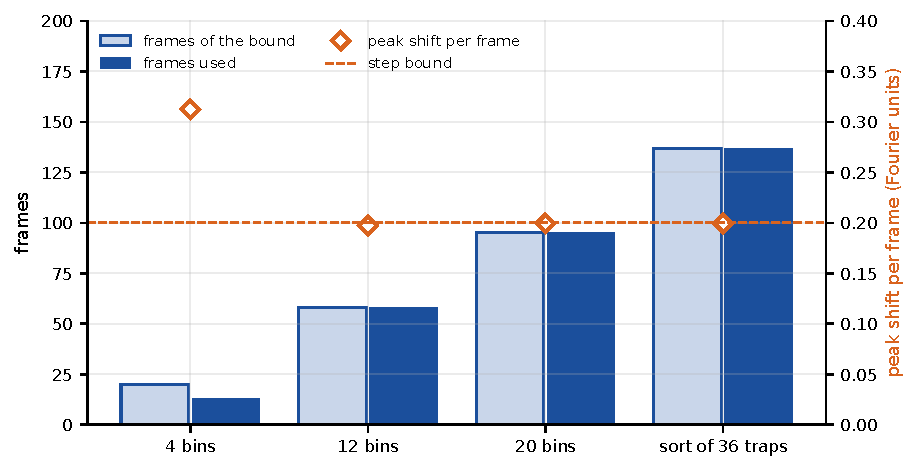
\includegraphics[width=\textwidth]{fig-bound.pdf}
\caption{Frames of the bound and frames used for the four moves of the experiments (acceptance task, two lattice moves and the sort), with the peak shift per frame of the frames used on the right axis; the dashed line is the step bound of the sequence.}
\label{fig:bound}
\end{figure}

Table~\ref{tab:bound} and Fig.~\ref{fig:bound} place the experiments against the equation. The three long moves are run at the frames of the bound and the peak shift per frame is at the bound, \claimStepFu{} Fourier units, up to rounding. The acceptance task is run at \parFrames{} frames, fewer than the \accFramesForMove{} of the bound, with a peak shift of \accPeakStep{} Fourier units, and meets $0.9$ on every seed; the sort at 25 frames has a peak shift of \cTenPeakEqual{} Fourier units and reaches no seed. The bound is therefore sufficient for the median and not necessary for a short move, and it is not sufficient for every seed of a long one.

\subsection{Cost in time}

\begin{figure}[t]
\centering
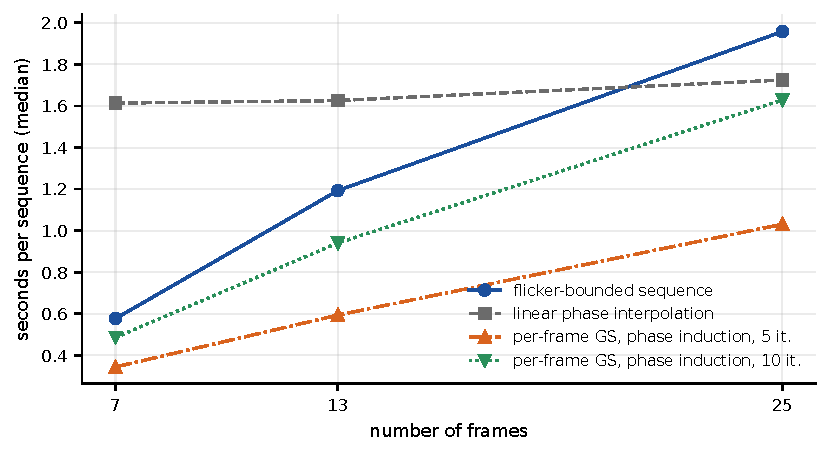
\includegraphics[width=\textwidth]{fig-seconds.pdf}
\caption{Seconds to compute one acceptance sequence of the four methods against the number of frames, median over \nSeedsTwo{} seeds, on the machine that produced the data; other jobs loaded the machine during part of the runs, so the values are an order of magnitude.}
\label{fig:seconds}
\end{figure}

Figure~\ref{fig:seconds} gives the seconds of one sequence. At \parFrames{} frames the median is \accBSecMed{} s for the sequence, \accKimFiveSecMed{} s for the per-frame method at \parKimIters{} iterations, \accKimTenSecMed{} s at ten and \accLpiSecMed{} s for linear phase interpolation, which runs two cold endpoint holograms and no iterations in between. The sequence is \secRatio{} times slower than the per-frame method at its own iteration count, which is the ratio of the iterations per frame, and \fpeval{round(\accBSecMean/\accKimTenSecMean,1)} times slower at equal work. The ratio of the seconds is slightly above the ratio of the iterations of the two sequences, \fpeval{round((\setupCold+(\parFrames-1)*\parFrameIters)/(\setupCold+(\parFrames-1)*\parKimIters),1)}, because the call that computes the proposed sequence also scores its transient ratio on the blend model, which the call of the baselines does not do; the seconds are therefore an upper estimate of the cost of the sequence itself, and they are not a measure of what a deployed implementation would take.

\subsection{Outcome of each hypothesis}

\begin{table}[t]
\centering\small
\caption{Outcome of each hypothesis of Table~\ref{tab:hyp} with the measurement that decides it, and the finding made after the results; ``held'' means the refuting condition did not occur.}
\label{tab:outcome}
\begin{tabular}{@{}l p{3.6cm} p{8.6cm}@{}}
\toprule
ID & Outcome & Measurement\\
\midrule
H1 & held & lowest seed \bTwoMin{}, linear phase interpolation highest seed \lpiMax{}; paired difference \diffTwoMean{} (\diffTwoCiLo{} to \diffTwoCiHi{})\\
H2 & held & largest step \accBStepMax{} rad against minimum \accKimFiveStepMin{} rad over seeds for the per-frame method; the sequence is smaller on every seed\\
H3 & refuted & reading of the dip at the default profile: \readThirteenKimFiveDip{} at \parKimIters{} iterations per frame, \readThirteenKimTenDip{} at \parFrameIters{}\\
H4 & held & reading of the per-frame spread: \readThirteenKimFiveSigma{} at \parKimIters{} iterations, \readThirteenKimTenSigma{} at \parFrameIters{}\\
H5 & held with failures & \longAMet{} of \longSeeds{} and \longBMet{} of \longSeeds{} seeds on the lattice moves, \cTenMet{} of \cTenSeeds{} on the sort\\
H6 & refuted by the majority rule & see Table~\ref{tab:ablation}: a majority of seeds stays at $0.9$ without the lock, with a lower mean and a wider range\\
H7 & held & see Table~\ref{tab:ablation}: no seed reaches $0.9$ without the per-frame optimization\\
H8 & held & median \bTwoMedSeven{} at 7 frames\\
F & finding made after the results, not a hypothesis & with the linear profile of the baselines the dip is read as \readProfileLinearKimFiveDip{} against the per-frame method at \parKimIters{} iterations, \readProfileLinearKimTenDip{} at \parFrameIters{} and \readProfileLinearLpiDip{} against linear phase interpolation (Table~\ref{tab:profile}); acceptance task only\\
\bottomrule
\end{tabular}
\end{table}

Table~\ref{tab:outcome} collects the outcomes of the eight hypotheses and, in its last row, the finding made after the results. Six hypotheses held, one of them with a qualification (H5, on a majority and not on all seeds), and two were refuted: H3, the sequence with its default profile is not as good on the dip as the published per-frame method at its own iteration count, and H6, by the majority rule the lock is not what keeps the dip above $0.9$ on the acceptance task, it acts on the phase step and on the spread of seeds. The finding made after the results is that with the constant-velocity profile of the baselines the sequence is read as better on the dip than every baseline on the acceptance task; it was not predicted, it was not run on the long moves or the sort, and it is reported as a finding and not as a revision of the outcome of H3. The deficit of the default on the dip belongs to its time profile and to a frame count outside its bound, not to the locked phases. The default frame count of the sequence, \parFrames{}, is the count that the source of linear phase interpolation uses for its sort, and it is below the count that the bound asks for the acceptance move.
